\documentclass{article}
\usepackage[a4paper]{geometry}

\geometry{a4paper, total={170mm,257mm} ,left=20mm ,right=20mm ,top=20mm}
\usepackage[table]{xcolor}
\usepackage{enumitem}
\usepackage{array}
\usepackage{tikz}
\usepackage{listings}
\usepackage{amsmath}
\usepackage{longtable}
\usepackage{multirow}
\usepackage{pgfplots}
\usepackage{minted}[cache=false]
\usepackage{subfig}
\usepackage{csvsimple}
\usepackage[english]{babel}
\usepackage[utf8]{inputenc}
\usepackage{fancyhdr}
\usepackage[hidelinks]{hyperref}
\usepackage{scrextend}
\usepackage{titlesec}
\usepackage{tabularray}
\usepackage[first=-20, last=10]{lcg}
\usepackage{hyperref}

\pagestyle{fancy}
\fancyhf{}
\rhead{\large \rightmark}
\lhead{\large Machine Learning Investigation}
\rfoot{\large Page \thepage}
\lfoot{\large Name: \\ Candidate Number: }

\newcounter{magicrownumbers}
\newcommand\rn{\stepcounter{magicrownumbers}\arabic{magicrownumbers}}
\newcommand\nrn{\stepcounter{magicrownumbers}\arabic{magicrownumbers}}
\newcommand{\random}{\rand\arabic{rand}}
\usetikzlibrary{matrix,shapes,arrows,positioning,chains}

\newcolumntype{C}[1]{>{\centering\let\newline\\\arraybackslash\hspace{0pt}}m{#1}}
\newcolumntype{L}[1]{>{\raggedright\let\newline\\\arraybackslash\hspace{0pt}}m{#1}}
\newcolumntype{M}[1]{>{\centering\arraybackslash}m{#1}}
\newcolumntype{N}{@{}m{0pt}@{}}

\newcommand{\pluseq}{\mathrel{+}=}
\newcommand{\greatereq}{\mathrel{>}=}
\newcommand{\lesseq}{\mathrel{<}=}
\newcommand{\minitab}[2][l]{\begin{tabular}{#1}#2\end{tabular}}

\newminted[pythoncode]{python}{frame=leftline,framesep=2mm,baselinestretch=1.2,linenos,fontsize=\footnotesize,breaklines}
\newminted[pseudocode]{markdown}{escapeinside=||,mathescape=true,frame=leftline,linenos,fontsize=\normalsize,breaklines}

\def\mathLarge#1{\mbox{\huge $#1$}}

\tikzset{block/.style={rectangle,draw,text width=10em,text badly centered,rounded corners}}

\titleformat{\section}
  {\normalfont\fontsize{12}{17}\sffamily\bfseries}
  {\thesection}
  {1em}
  {}

\titleformat{\subsection}
  {\normalfont\fontsize{12}{17}\sffamily\bfseries}
  {\thesubsection}
  {1em}
  {}

\titleformat{\subsubsection}
  {\normalfont\fontsize{11}{14}\sffamily\bfseries}
  {\thesubsubsection}
  {1em}
  {}

\definecolor{Water}{RGB}{18, 89, 144}
\definecolor{Beach}{RGB}{245, 234, 146}
\definecolor{Grass}{RGB}{26, 148, 49}
\definecolor{Mount}{RGB}{136, 140, 141}
\definecolor{Tree}{RGB}{13, 92, 28}
\definecolor{Player}{RGB}{233, 182, 14}
\definecolor{Enemy}{RGB}{207, 2, 2}

\begin{document}

\begin{titlepage}
    \begin{center}
        \vspace*{3cm}
        {\Huge \textbf{An Investigation into Machine Learning through the Simulation of Human Survival}} \\
        \vspace{1cm}
        {\Large Computer Science NEA}
        
        \vfill
        
        \large
        \textbf{Name:} \\
        \textbf{Candidate Number:} \\
        \vspace{0.2cm}
        \textbf{Centre Name:} Barton Peveril College\\
        \textbf{Centre Number:} 58231\\
        \pagebreak
    \end{center}
\end{titlepage}

\large

\setcounter{tocdepth}{5}
\tableofcontents

\begin{flushleft}
    \huge
    \textbf{2. Analysis}
    \vspace{0.1cm}

    \Large
    \begin{enumerate}
        \item {\Large Statement of Investigation} \\
            \large
            \vspace{0.2cm}
            I plan to investigate Machine Learning by developing a survival simulation environment 
            in which a character will be controlled by a Machine Learning algorithm. The survival simulation will 
            present multiple challenges such as dynamic threats towards the agent in order to provide a complex 
            problem for it to solve. The key question I aim to answer with this investigation is:

            \vspace{0.3cm}

            \begin{center}
            \textbf{Can you train a Machine Learning algorithm to survive in a pseudo random, open-world environment?}
            \end{center}

            \vspace{0.3cm}

            I find this question to be quite interesting because there is multiple layers of complexity to it, 
            with several different problems to solve. Answering the question will require me to dive headfirst into 
            Machine Learning picking things up as fast as possible.

        \vspace{1cm}
        \item {\Large Background} \\
            \vspace{0.2cm}
            I am investigating this area of Computer Science because I've been interesting in attempting a form of
            Machine Learning for a while now but havent had a reason to dive into it. Machine Learning is an evolving
            field, with mere infinite applications such as Image Recognition, Chat Bots, Self Driving Cars, 
            etc. I feel as though my project will be sufficiently advanced enough to expand my knowledge of the subject.
            It will require lots of research, planning, and design work in order to successfully fulfil my Technical
            Solution. \\
            \vspace{0.2cm}

        \vspace{1cm}
        \item {\Large Expert} \\
            \vspace{0.2cm}
            For my expert I approached one of my friends, Ben, who has prior experience with Machine Learning. He has
            created his own Hand Written Digit Recognition Network before, along with using Python Libraries such as 
            \textit{PyTorch} to train an agent to play the game \textit{Flappy Bird}, among other ML projects. He has 
            a much better understanding of Machine Learning than me currently, so hopefully he will be a good resource 
            as I develop my project. \\
            \vspace{0.2cm}
            He has agreed to answer some questions for my Interview once I have completed my Initial Investigation.

        \vspace{1cm}
        \item {\Large Initial Research} \\
            \begin{enumerate}
                \item {\Large Existing Investigations} \\
                    \begin{enumerate}
                        \item {\large \textbf{Crafter}}
                            In my research on the Internet I discovered a project called $Crafter$.
                            
                            \centerline{\texit{https://github.com/danijar/crafter}}

                            Crafter is described to be \textit{"Benchmarking the Spectrum of Agent Capabilities"}, and is utlised
                            in conjunction with Machine Learning Algoriths such as $DreamerV2$, $PPO$ and $Rainbow$. Crafter poses significant
                            challenge towards its Player, requiring high levels of generalisation, long-term reasoning, and complex 
                            problem solving. If the machine Learning algorithm in question fails to achieve one of these aspects it will 
                            struggle to full "Solve" the simulation. \\

                            \vspace{0.2cm}

                            High levels of generalisation are required when training a Machine Learning algorithm, if this is not achieved then
                            your network will only lend itself to a single Dataset/Problem. An example of this would be training a network used
                            to recognise hand written digits on only one way of writing 4's, if presented with an input for a different type of 
                            4 it may not recognise it and identify it incorrectly. \\
                            
                            \vspace{0.2cm}

                            Long-Term reasoning is a complex problem to solve in the context of Machine Learning, current Machine Learning models
                            struggle to deal with this problem. This is dealt with by using algorithms built to mimic "memory". A common 
                            implementation of this is Experience Replay which stores states in a queue, and relearns from it after every N ammount
                            of steps. \\

                            \vspace{0.2cm}

                            A complex reward and action system may take time for an algorithm to learn but it certainly is possible with current
                            Machine Learning Models. Crafter utilises a complex action system with a flow chart determining which Action can be taken
                            given the current state of the simulation. Below is shown the Complex Flow Chart of Actions: \\

                            \vspace{0.2cm}
                            \begin{center}
                                \includegraphics[width=8cm]{Images/Initial Research/CrafterComplexActionSystem.PNG}
                                Complex action system as shown in the Paper "Benchmarking the Spectrum of Agent Capabilities" \\
                            \end{center}
                            \vspace{0.2cm}

                            While I would love to create a simulation similar to crafter, it is very complex and would take a long time to develop. Yet
                            would not net many marks in the process.

                            \vspace{0.2cm}
                        \item {\large \textbf{Minecraft}}
                            Minecraft is a \textit{very} popular Game. It's a sandbox game, meaning that the player can do almost anything they want.
                            It has infinite terrain generation, and explicity uses Perlin Noise, and is generated from a seed. The seed determines
                            all the terrain generation, loot tables, random structures, caves, etc. Two seeds next to eachother will also be wildly
                            different. \\
                            
                            \vspace{0.2cm}

                            First it starts off on a very broad level, painting a basic topographical map of the world. It then adds finer detail
                            of noise in the form of Biomes, Shrubbery and Generated Structures. \\

                            \includegraphics{Images\Initial Research/MCTerrainGeneration.jpg}
                            \includegraphics{Images\Initial Research/MCStructureGeneration.jpg}

                        \item {\large \textbf{Conways Game of Life}}

                \end{enumerate}

                \item {\Large Algorithms and Potential Data Types} \\
                    \large
                    \vspace{0.2cm}
                    
                    {\Large Neural Network and Matrices} \\
                    As part of developing a Machine Learning Algorithm, I will need to implement a Matrix class in order to
                    implement a neural network. Matrices are commonly used to represent individual layers of a network. Along
                    with making calculations much easier, condensing them into performing operations on matrices, rather than
                    nested using nested for loops and lists. As part of my Initial Research I have taken the time to understand
                    how a Neural Network functions, it turns out I have already learned most of the Maths needed to understand
                    how it works in my A Level Maths and Further Maths courses. \\
                    \vspace{0.2cm}
                    A Neural Network functions as a series mathematical equations used to recognise relationships between inputs
                    and desired outputs. They take in a Vector of Input Data, and output a Vector of Output Data. They can be
                    in simple terms as a function: $N(x)$ where: $\{x \in V, N(x) \in V\}$. The functions name in this case is
                    Forward Propagation. 
                    \vspace{0.2cm}
                    We form a Neural Network with multiple layers of Nodes, the layers being referred to as the Input Layer, 
                    Hidden Layer/s and Output Layer. In this case each Node is connected to every Node in the previous layer and
                    the following layer. In the below image is represented a Neural Network with a layer structure of $[3, 5, 2]$.

                    \vspace{0.1cm}
                    \centerline{\includegraphics[width=10cm]{Images/Initial Research/NeuralNetworkExample.png}}

                    Each connection, otherwise known as an Arc or Edge, has an associated weight. Along with every output of a
                    layer having an associated Bias. These are used to compute the outcome of a network.
                    \vspace{0.2cm}
                    Forward Propagation is used to compute the outcome of a network, it has a general form and uses 
                    Matrix Multiplication and Addition to achieve this.
                    \vspace{0.2cm}
                    
                    \begin{center}
                        $
                        S^{(L)} = 
                        \begin{bmatrix}
                        s^{(L)}_{0} \\
                        s^{(L)}_{1} \\
                        \vdots      \\
                        s^{(L)}_{n} 
                        \end{bmatrix}
                        = 
                        \begin{bmatrix}
                        w^{(L-1)}_{0,0} & w^{(L-1)}_{0,1} & \hdots  & w^{(L-1)}_{0,m} \\
                        w^{(L-1)}_{1,0} & w^{(L-1)}_{1,1} & \hdots  & w^{(L-1)}_{1,m} \\
                        \vdots          & \vdots          & \ddots  & \vdots          \\
                        w^{(L-1)}_{n,0} & w^{(L-1)}_{n,1} & \hdots  & w^{(L-1)}_{n,m} \\
                        \end{bmatrix}
                        \begin{bmatrix}
                        a^{(L-1)}_{0} \\
                        a^{(L-1)}_{1} \\
                        \vdots      \\
                        a^{(L-1)}_{n} 
                        \end{bmatrix}
                        +
                        \begin{bmatrix}
                        b^{(L)}_{0} \\
                        b^{(L)}_{1} \\
                        \vdots      \\
                        b^{(L)}_{n} 
                        \end{bmatrix}
                        $ 
                    \end{center}
                    
                    \begin{center}
                        $
                        \sigma(S^{(L)})
                        =
                        \sigma\left(
                        \begin{bmatrix}
                        s^{(L)}_{0} \\
                        s^{(L)}_{1} \\
                        \vdots      \\
                        s^{(L)}_{n} 
                        \end{bmatrix}
                        \right)
                        =
                        \begin{bmatrix}
                        \sigma(s^{(L)}_{0}) \\
                        \sigma(s^{(L)}_{1}) \\
                        \vdots              \\
                        \sigma(s^{(L)}_{n}) 
                        \end{bmatrix}
                        $ 
                    \end{center}
                    
                    \vspace{0.2cm}
                    We then apply an activation function as shown above, in this case we will apply the Sigmoid function: $\sigma(x)$ to $S^{(L)}$. The Sigmoid function is a Mathematical Function which \textit{squishes} values between 0 and
                    1. Shown Below:
                    
                    \begin{center}
                        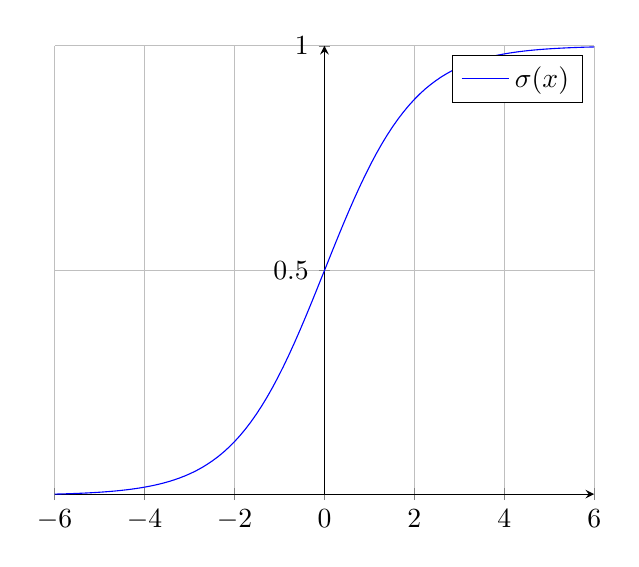
\begin{tikzpicture}[declare function={sigma(\x)=1/(1+exp(-\x));}]
                        \begin{axis}%
                        [
                            grid=major,     
                            axis x line=bottom,
                            ytick={0,.5,1},
                            ymax=1,
                            axis y line=middle,
                            samples=100,
                            domain=-6:6,
                            range=0:1
                            legend style={at={(1,0.9)}}     
                        ]
                            \addplot[blue,mark=none]   (x,{sigma(x)});
                            \legend{$\sigma(x)$}
                        \end{axis}
                        \end{tikzpicture}
                    \end{center}

                    Matrices can be used for all parts of a Neural Network implementation, and will prove very useful in my Technical
                    Solution. \\
                    \vspace{0.5cm}
                    
                    \pagebreak
                    {\Large Procedural Generation} \\
                    For my project I am going to have to procedurally generate 2d terrain, while researching this I came across a few algorithms
                    which seemed to be able to do this pretty well. I will compare two algorithms I discovered below.
                    
                    \begin{flushleft}
                        \begin{tabular}{| C{6cm} | C{6cm} |}
                            \hline
                            {\Large Post-Processing Algorithms} & {\Large Perlin Noise} \\
                            \hline
                            I discovered two post processing algorithms often used for simple 2d terrain generation. 1 Averages squares 
                            around the selected square, and the other pulls it up or down the gradient its currently on.
                            I find these interesting because they're relatively simple, and I'm not quite sure whether they will produce good results or not. 
                            \vspace{0.2cm}\linebreak
                            So it would be interesting to test out implementing these in my prototype.
                            &
                            Perlin Noise is an algorithm developed by Ken Perlin for use in the digital generation of noise.
                            This noise can be combined to create \textit{realistic} looking height maps for world generation.
                            Perlin Noise retains continuity and is seeded so the generation can be entirely controlled.
                            By "retains continuity" I mean that you can sample the same point and retrieve the same value. 
                            \vspace{0.2cm}\linebreak
                            
                            If I was to implement Perlin noise it would take longer, but also might end up with a better result
                            due to it being more widely used. It's a trade-off between time to implement and desired result. \\
                            \hline
                        \end{tabular}
                    \end{flushleft}
                    
                    I also discovered an algorithm called Poisson Disc Sampling, this can be used to sample random points 
                    in N dimensional space. It takes in 2 values, the R and K value, these values determine the output of
                    the function. The R values is the minimum distance a point has to be from another, randomly placed point
                    which hasn't been selected yet. If the distance between any existing points is less than R, the point
                    will be rejected and another will be selected. The K value determines how many rejected are needed before 
                    the algorithm will stop attempting to choose a new point.
                    
                    \vspace{0.5cm}
                    {\Large Proposed Programming Language and Associated Libraries} \\
                    When selecting a Programming Language and associated Graphical Libraries I took into consideration a few options.
                    Below I have weighed up 3 options for Programming Language, along with 2 graphical libraries per language
                    
                    \begin{flushleft}
                        \begin{longtable}{|M{2cm}|M{2cm}|M{8cm}|}
                        \hline
                        Proposed Solution & \multicolumn{2}{M{10cm}|}{Benefits and Downsides of Proposed Solution} \\
                        \hline
                            Python & \multicolumn{2}{M{10cm}|}{Python is the first thought which comes to mind when I think about programming, 
                            it is my favourite language and I'm yet to find anything which I prefer. Its very versatile and great
                            for rapid prototyping, the dynamic typing makes It great for coding quickly without worrying too
                            much about whether you're using a \textit{float32 or float64}. It also has hundreds of libraries
                            and is very well supported by its developers and the community.}\\
                        \hline
                            \multirow{2}*{\minitab[c]{Python \\ Graphical \\ Libraries}} & Pygame & Pygame is a highly customizable and well developed binding of
                            \textit{Simple DirectMedia Layer} (SDL) Library. It has a full set of 2d drawing tools, along with keyboard and audio
                            capabilities. I have lots of experience with Pygame so I already have code which I can take from, which will speed up
                            development when dealing with the Pygame library.\\
                        \cline{3-3}
                            &Tkinter & Tkinter provides an interface to the standard \textit{Tcl/Tk GUI Toolkit}, which is available
                            for most platforms, this makes it highly versatile. Though as my project is not intended as a software
                            package I dont see this as being an incredibly big selling point. Tkinter will serve mostly the same
                            purpose as Pygame but give me easier options for Graphical Input, I dont currently plan to add GUI so 
                            this feature isnt neccesary.\\
                        \hline
                            C\# & \multicolumn{2}{M{10cm}|}{C\# is my second favourite language, I have plenty of experience with it from developing games
                            with Unity. Its faster than Python and is less abstracted, but this speed isn't necessarily required
                            for my project. With C\# I could utilise the \textit{Unity Game Engine} for my project, but then
                            I might end-up relying on builtin types and functions rather than developing my own.}\\
                        \hline
                    \end{longtable}

                    \pagebreak
                    \begin{longtable}{|M{2cm}|M{2cm}|M{8cm}|}
                        \hline
                        Proposed Solution & \multicolumn{2}{M{10cm}|}{Benefits and Downsides of Proposed Solution} \\
                        \hline
                            \multirow{2}*{\minitab[c]{C\# \\ Graphical \\ Libraries}} & Windows Forms & Windows Forms is a relatively simple drag drop
                            interface for designing your own applications. I've never used it before but I could utilise it with C\# to create my project.
                            I belive it might be a bit overkill for my needs though, as it includes many, many UI features which I will have no use for.\\
                        \cline{3-3}
                            & WPF & WPF or \textit{Windows Presentation Foundation} is a versatile development platform for desktop applications.
                            It is relatively versatile in its uses and utilises XAML and is the UI Language of Windows Platforms. XAML would be a
                            new language for me to learn but I have experience with HTML so I dont believe it would be too difficult.
                            The platform would provide a stable base to my project.\\
                        \hline
                            Rust & \multicolumn{2}{M{10cm}|}{Rust is low level language designed for speed and efficiency, I started using it recently
                            as a side hobby and would like to use it more in future projects of mine. Though I feel like it may be a bit overkill for a Computer 
                            Science NEA, with it often being used for server side applications rather than general purpose applications.}\\
                        \hline
                            \multirow{2}*{\minitab[c]{Rust \\ Graphical \\ Libraries}} & Piston2d & Piston2d is a feature complete 2d graphics library which utilises OpenGl,
                            I've worked with it briefly before and I believe it would be a good option over Pixels if I needed more complex drawing
                            methods.\\
                        \cline{3-3}
                             & Pixels & Pixels is a lightweight 2d graphics library designed to simply push pixels to the screen, Its relatively simple
                             and ive used it for making a simple \textit{Falling Sand Game} before, could be a good little option if I wanted to develop
                             a lightweight solution.\\
                        \hline
                        \end{longtable}
                    \end{flushleft}
                    
                \item {\Large Interview} \\
                    \large
                    \vspace{0.2cm}
            \end{enumerate}

            \pagebreak
        \item {\Large Prototype} \\
            \large
            \vspace{0.2cm}
            Before starting my Prototype I had to decide upon a short list of objectives I wanted to 
            complete/investigate as part of it. These boiled down to a few things:

            \vspace{0.2cm}
            \begin{enumerate}
                \item Terrain Generation
                \item Displaying the Generated Terrain using a Graphics Library
                \item Matrix and Vector implementation
            \end{enumerate}
            \vspace{0.2cm}

            For my Prototype, I first created a GitHub Repository, available here: 
            
            \vspace{0.1cm}
            \centerline{\textit{https://github.com/TheTacBanana/CompSciNEAPrototype}}
            \vspace{0.1cm}

            I had created a hierarchy of importance for development in my head, visualized using this flow diagram:

            \begin{center}
                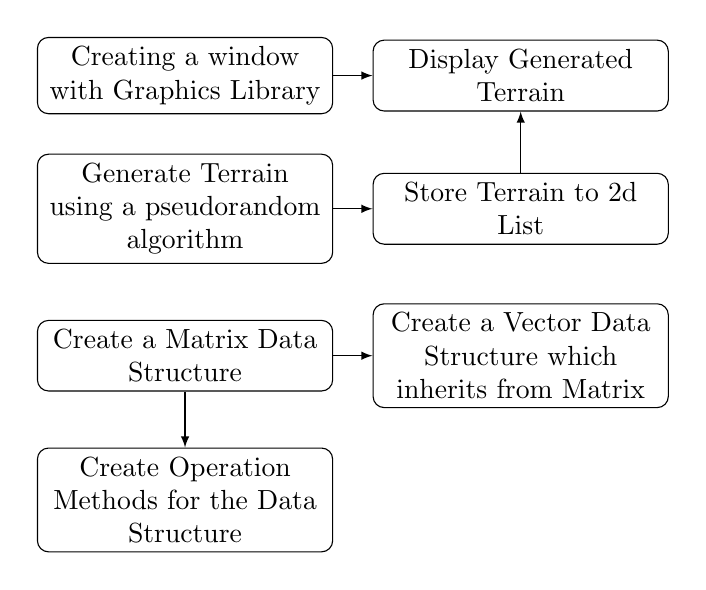
\begin{tikzpicture}
                    \matrix (m)[matrix of nodes, column  sep=0.5cm,row  sep=0.5cm, align=center, nodes={rectangle,draw, anchor=center} ]{
                        |[block]| Creating a window with Graphics Library &  |[block]| Display Generated Terrain \\   
                        |[block]| Generate Terrain using a pseudorandom algorithm &  |[block]| Store Terrain to 2d List \\
                        |[block]| Create a Matrix Data Structure & |[block]| Create a Vector Data Structure which inherits from Matrix \\
                        |[block]| Create Operation Methods for the Data Structure & \\
                    };
                    \path [>=latex,->] (m-1-1) edge (m-1-2);
                    \path [>=latex,<-] (m-1-2) edge (m-2-2);
                    \path [>=latex,->] (m-2-1) edge (m-2-2);
                    \path [>=latex,->] (m-3-1) edge (m-3-2);
                    \path [>=latex,->] (m-3-1) edge (m-4-1);
                \end{tikzpicture}
            \end{center}

            I decided to use Python for developing my Prototype, this seemed like a good fit due to me 
            having lots of experience with the language. Python is a Dynamically Typed and Interpretted 
            language which makes it versatile for protyping and fast, iterative development.
            
            \vspace{0.5cm}

            {\Large Terrain Generation and Displaying} \\
            \vspace{0.25cm}

            Starting from the begining of my hierarchy I installed Pygame using \textit{pip} and started creating a window.
            This was a relatively simple task only taking a few lines:
            \vspace{0.5cm}

            \normalsize
            \begin{minted}[frame=leftline,framesep=2mm,baselinestretch=1.2,fontsize=\footnotesize,linenos]{python}
import pygame

simSize = 128
gridSize = 2

window = pygame.display.set_mode((simSize*gridSize, simSize*gridSize))
pygame.display.set_caption("Procedural Generation")

running = True
while running == True:
  for event in pygame.event.get():
    if event.type == pygame.QUIT:
      running = False
            \end{minted}

            \vspace{0.5cm}

            \large
            This creates a window like this: \\ 
            \vspace{0.5cm}
            \centerline{\includegraphics{Images/Prototype/CreateWindowExample.PNG}}

            \vspace{0.5cm}

            Following the hierarchy I then added noise generation by generating random numbers and 
            assigning them to a 2d List. Shown here: 
            
            \begin{minted}[frame=leftline,framesep=2mm,baselinestretch=1.2,fontsize=\footnotesize,linenos]{python}
def GenerateMap(self, seed):
    random.seed(seed)
    for y in range(0, self.arraySize):
        for x in range(0, self.arraySize):
            self.heightArray[x][y] = round(random.random(),2)
            \end{minted}

            \vspace{0.5cm}

            \large
            After creating some code to draw squares based upon the random value, I ended up with this 
            random array of Black-White squares:\\
            \vspace{0.5cm}
            \centerline{\includegraphics{Images/Prototype/RandomNoiseExample.PNG}}

            \vspace{0.5cm}

            This was a good start, but didnt really look like terrain yet. As part of my research I came 
            across simple algorithms to turn random noise into usable 2d terrain. I decided to implement
            these algorithms. They are relatively short and didnt take too much time to implement. I've
            named the two algorithms UpDownNeutralGen and Average.

            \vspace{1cm}

            {\large UpDownNeutralGen Method} \\
            \vspace{0.25cm}

            The UpDownNeutralGen method takes a tile, and considers every tile around it. It sums the tile 
            which are greater than, less than, or within a certain range of the tile height. And then pulls
            the selected tile in the direction which has the highest precedence. As an example, here are some
            randomly generated values:

            \begin{center}
                \begin{tabular}{| C{0.75cm} | C{0.75cm} | C{0.75cm} |}
                    \hline
                    0.71 & 0.19 & 0.3 \\ [0.75cm]
                    \hline
                    0.46 & 0.26 & 0.82 \\ [0.75cm]
                    \hline
                    0.63 & 0.35 & 0.05 \\ [0.75cm]
                    \hline
                \end{tabular}
            \end{center}

            If we count the surrounding values into corresponding Higher, Lower and Neutral we get: \\

            \begin{center}
                \begin{tabular}{| M{2cm} | M{2cm} | M{2cm} |}
                    \hline
                    Higher & Lower & Neutral \\ [0.25cm]
                    \hline
                    4 & 1 & 3 \\ [0.25cm]
                    \hline
                \end{tabular}
            \end{center}

            \vspace{0.5cm}

            This leads us to calculating the \textit{pullValue}, respectively for each case:
            \begin{center}
                $Up -> pullValue = upTiles * 0.09$ \\
                $Down -> pullValue = upTiles * -0.08$ \\
                $Neutral -> pullValue = 0$ \\
                \vspace{0.5cm}
                $Value[x][y] \pluseq pullValue$\\
            \end{center}
            
            \vspace{0.5cm}

            We then add the pullValue to the original square value, leaving us with the updated value. The code for 
            this shown under the Prototype Code Header.
            \vspace{0.5cm}

            {\large Average Method}
            \vspace{0.25cm}

            The Average method takes a tile and considers every tile around it, this time instead of looking at the
            differences, it creates an average from the 8 surrounding tiles. It then sets the selected tile to this
            average value. As an example, here are some randomly generated values:

            \begin{center}
                \begin{tabular}{| C{0.75cm} | C{0.75cm} | C{0.75cm} |}
                    \hline
                    0.83 & 0.93 & 0.64 \\ [0.75cm]
                    \hline
                    0.07 & 0.38 & 0.21 \\ [0.75cm]
                    \hline
                    0.33 & 0.94 & 0.95 \\ [0.75cm]
                    \hline
                \end{tabular}
                \vspace{0.25cm}

                Summing these and dividing by the total grants us the average:

                \[
                \frac{0.83 + 0.93 + 0.64 + 0.07 + 0.38 + 0.21 + 0.95 + 0.33 + 0.94}{9} = 0.586
                \]
                $Value[x][y] = 0.586$
            \end{center}
            \vspace{0.25cm}

            The code for this shown under the Prototype Code Header.

            \vspace{1cm}

            {\large Finished Terrain Generation} \\
            \vspace{0.25cm}

            Overall I am happy with the Terrain generation, though I feel as if it could be improved to look more realistic.
            The difference between the original random noise and the Colour Mapped Terrain looks so much better.

            \begin{center}
                \includegraphics[width=6cm]{Images/Prototype/Seed420 Grayscale.png}
                \includegraphics[width=6cm]{Images/Prototype/Seed420 Colour.png} 
            \end{center}
            
            \vspace{1cm}
            {\Large Matrix Data Structure} \\
            \vspace{0.25cm}

            As part of my Matrix Class I made a list of operations which would be key to a Matrix Class, along with being useful
            for Machine Learning. A Matrix is an abstract data type, commonly used in Maths, but has practical uses in the world
            of Computer Science. It holds a 2d array of values such as: \\ 
            \begin{center}
            $\begin{pmatrix}
                a & b\\
                c & d
            \end{pmatrix}$ 
            $\begin{pmatrix}
                a & b & c \\
                d & e & f \\
                g & h & i 
            \end{pmatrix}$ 
            $\begin{pmatrix}
                a \\
                b \\
                c  
            \end{pmatrix}$ 
            $\begin{pmatrix}
                a & b & c & d\\
                e & f & g & h
            \end{pmatrix}$ 
            \end{center}
            The values in a Matrix can be manipulated using common operations such as $+ - *$ as long as the orders of the 2 Matrices
            match up. Along with other, non-standard operations which have other purposes.

            \vspace{0.25cm}
            As part of my Matrix Class, I implemented the following operators:
            \begin{enumerate}
                \item Addition/Subtraction \\
                    Implementing Addition didnt take too long, I utilised a nested for loop to iterate over every value in both Matrices.
                    Adding the two values together into a temporary Matrix which the method then returned. 
                    \vspace{0.25cm}
                    \begin{center}
                        $\begin{pmatrix}
                            a & b\\
                            c & d
                        \end{pmatrix} +
                        \begin{pmatrix}
                            e & f\\
                            g & h
                        \end{pmatrix} =
                        \begin{pmatrix}
                            a+e & b+f\\
                            c+g & d+h
                        \end{pmatrix}$
                    \end{center}
                    \vspace{0.25cm}

                \item Multiplication \\
                    Multiplication of Matrices is slightly more complicated, it is of $O(n^3)$ complexity, utilising a triple nested for loop.
                    It multiplies the row of a $M1$, by the column in $M2$. Summing the calculation into the element in the new Matrix $M3$. \\
                    
                    \vspace{0.25cm}
                    \begin{center}
                        $\begin{pmatrix}
                            a & b\\
                            c & d
                        \end{pmatrix} *
                        \begin{pmatrix}
                            e & f\\
                            g & h
                        \end{pmatrix} =
                        \begin{pmatrix}
                            a*e + b*g & a*f + b*h\\
                            c*e + d*g & c*f + d*h
                        \end{pmatrix}$
                    \end{center}
                    There is also Scalar Multiplication which multiples each value of a Matrix by the Scalar.
                    \begin{center}
                        $k *
                        \begin{pmatrix}
                            a & b\\
                            c & d
                        \end{pmatrix} =
                        \begin{pmatrix}
                            ka & kb\\
                            kc & kd
                        \end{pmatrix}$
                    \end{center}
                    \vspace{0.25cm}

                \item Determinant \\
                    Calculating the Determinant of an NxN Matrix is a recursive algorithm. With the base case being the Determinant of a 2x2
                    Matrix. When calculating the Determinant of a 3x3 Matrix you create a Matrix of Cofactors, and multiply each 
                    value by the corresponding value in the Sin Matrix (\textit{Formed from repeating 1's and -1's}). Summing the values from
                    a singular Row or Column will then give you the Determinant. For a 4x4 you simply calculate the Determinant of the corresponding
                    3x3's to get the Cofactors.
                    
                    \begin{center}
                        $
                        \begin{vmatrix}
                            a & b\\
                            c & d
                        \end{vmatrix} = 
                            a*d - b*c
                        $
                    \end{center}
                    \vspace{0.25cm}
                    \begin{center}
                        $\begin{vmatrix}
                            a & b & c \\
                            d & e & f \\
                            g & h & i 
                        \end{vmatrix}  = a*
                        \begin{vmatrix}
                            e & f\\
                            h & i
                        \end{vmatrix}
                        -b*
                        \begin{vmatrix}
                            d & f\\
                            g & i
                        \end{vmatrix}
                        +c*
                        \begin{vmatrix}
                            d & e\\
                            g & h
                        \end{vmatrix}$
                    \end{center}
                    \vspace{0.25cm}

                \item Dot Product \\
                    The Dot Product occurs between two vectors, and can be used to calculate the angle between them. 
                    Its a relatively simple operation only taking a few lines of code.
                    \begin{center}
                        $
                        \begin{pmatrix}
                            a \\
                            b \\
                            c
                        \end{pmatrix} .
                        \begin{pmatrix}
                            d \\
                            e \\
                            f
                        \end{pmatrix} = 
                        a*d + b*e + c*f$
                    \end{center}
            \end{enumerate}

            All code is available under the Prototype Code Header.
            
            \vspace{1cm}
            {\Large Prototype Evaluation} \\
            \vspace{0.25cm}

            Overall I am happy with my prototype, though I feel like some parts need to be improved. I did meet my 
            objectives for my prototype but there were improvements which can me made when I create my Technical Solution. 
            Namely the Terrain Generation along with the Matrix class. I feel that Perlin noise would be a better alternative
            to the two algorithms I used. In theory it should produce better results, and also provice more marks for 
            complexity. My Matrix class could be rewritten to be more efficient, along with using operator overloading, which
            I didnt know Python could do at the time. I also feel like having vector inherit from matrix is relatively pointless,
            there is no need for it when I could just use 1 wide Matrices.

            \pagebreak
        \item {\Large Objectives} \\
            \large
            Taking into account my Prototype and Interview, I have formed a list of objectives I feel to be most 
            appropriate for my Investigation.
            If all completed they will form a complete solution which will answer my Investigations question.
            Below is the list of objectives split into 6 key sections:

            \begin{enumerate}
                \item User Input
                    \begin{enumerate}
                        \item Read Parameters from a Json formatted file
                        \item Check Parameters fall within a certain range to prevent errors
                        \item Give user option to load Neural Network Training progress
                    \end{enumerate}
                \item Simulation
                    \begin{enumerate}
                        \item Utilise Perlin Noise to generate a 2d List of terrain heights
                        \item Store Terrain Heights in a Tile Data Type
                        \item Utilise Threading to generate Terrain Faster
                        \item Display terrain to a pygame window
                        \item Map ranges of terrain heights to specific colour bands
                        \item Utilise Poisson Disc Sampling to generate objects for the Agent to interact with
                        \item Implement enemies which use basic pathfinding to traverse towards the player
                        \item Generate multiple enemies upon starting the simulation
                        \item Allow the enemies to attack the Agent
                    \end{enumerate}   
                \item Agent
                    \begin{enumerate}
                        \item Implement Movement options for the Agent
                        \item Implement the ability to pick up the generated Objects
                        \item Implement the ability to attack the generated enemies
                        \item Create methods to sample the terrain around the Agent
                        \item Create methods to convert the sampled Tiles into a grayscale input vector for a neural network
                        \item Create reward methods to reward the agent given the terrain samples and action
                    \end{enumerate}   
                \item Matrix Class
                    \begin{enumerate}
                        \item Implement a Dynamic Matrix Class with appropriate Operations such as:
                            \begin{enumerate}
                                \item Multiplication
                                \item Addition
                                \item Subtraction
                                \item Transpose
                                \item Sum
                                \item Select Row/Column
                            \end{enumerate}
                        \item Create appropriate errors to throw when utilising methods the incorrect way
                    \end{enumerate}   
                \item Deep Q Learning
                    \begin{enumerate}
                        \item Dynamically create a Dual Neural Network model based upon loaded parameters
                        \item Implement an Abstract Class for Activation Functions
                        \item Implement Activation Functions inheriting from the Abstract Class such as:
                        \begin{enumerate}
                            \item ReLu
                            \item Sigmoid
                            \item SoftMax
                        \end{enumerate}
                        \item Create methods to Forward Propagate the neural network
                        \item Create methods to calculate the loss of the network using the Bellman Equation
                        \item Create methods to Back Propagate calculated error through the neural network
                        \item Create methods to update weights and biases within the network to converge on a well trained network
                        \item Utilise the outlined Matrix class to perform the mathematical operations in the specified methods
                        \item Implement Load and Save Methods to save progress in training
                        \item Implement a Double Ended Queue/Deque Data Type
                        \item Implement Experience Replay utilising the Deque Data Type to increase training accuracy
                    \end{enumerate}   
                \item Data Logger
                    \begin{enumerate}
                        \item Be able to create a Data Logger class to log data points across training
                        \item Be able to create a Data Structure for the Data Logger
                        \item Allow multiple types specified types for a single parameter
                        \item When adding a new Data Point the Logger will check it to make sure it matches the given Data Structure
                        \item Implement a Heap Data Type
                        \item Implement a Heap sort using the Heap Data Type
                        \item Be able to sort by a parameter in the Data Structure
                        \item Be able to select a single parameter from the data points
                        \item Implement Load and Save Functions to save progress during training
                    \end{enumerate}   
            \end{enumerate}
    \end{enumerate}
\end{flushleft}

\begin{flushleft}
    \huge
    \textbf{3. Design}

    \Large
    \begin{enumerate}
        \item {\Large System Flow Charts} \\
            \large
            \vspace{0.2cm}
            Below is shown the Flow Chart Overview of my Entire Project. This flowchart is very abstracted without going into
            the fine detail of each Process. \\
            
            \vspace{0.5cm}
            \centerline{\includegraphics[width=\textwidth]{Images/Design/NEA Flow Chart.png}}
            \vspace{0.5cm}

            

        \item {\Large Class Diagrams}
            \large
            \vspace{0.2cm}

        \item {\Large Description of Algorithms}
            \large
            \vspace{0.2cm}
            \begin{enumerate}[label=\arabic*)]
                \item Matrix Addition \\
                This algorithm is a Mathematical Operation to add 2 Matrices together. To Add together 2 Matrices their Orders
                must be the same. To perform the Operation you must Sum each element in Matrix A with the corresponding element 
                in Matrix B, placing the result of each Sum in the resultant Matrix.

                \vspace{0.5cm}
                \item Matrix Subtraction \\
                This algorithm is a Mathematical Operation to subtract 2 Matrices. To Subtract 2 Matrices their Orders
                must be the same. To perform the Operation you must Sum each element in Matrix A with the negative of the 
                corresponding element in Matrix B, placing the result of each Sum in the resultant Matrix.

                \vspace{0.5cm}
                \item Matrix Multiplication \\
                This algorithm is a Mathematical Operation to find the product of 2 Matrices. To Multiply 2 Matrices
                the number of Columns in the Matrix A must be equal to the number of Rows in Matrix B. Where Matrix A has
                dimensions of $m$ x $n$ and Matrix B has dimensions of $j$ x $k$, the resultant Matrix will have dimensions of 
                $n$ x $j$. To Multiply two Matrices, the algorithm performs the Dot Product between the Row in Matrix A and the 
                corresponding Column in Matrix B. The Dot Product is the Sum of the Products of corresponding elements.

                \vspace{0.5cm}
                \item Matrix Scalar Multiplication \\
                This algorithm is a Mathematical Operation to find the product between a Matrix and a Scalar.
                The result can be found by Multiplying each element of the Matrix by the Scalar Value to form the Resultant 
                Matrix.
                
                \vspace{0.5cm}
                \item Matrix Hadamard Product \\
                This algorithm is a Mathematical Operation to another way to find the product between 2 Matrices. Instead of
                applying the Dot Product between Rows and Columns, you find the product between each element in Matrix A
                with the corresponding element in Matrix B, placing the result in the resultant Matrix. This is very epic gamer

                \vspace{0.5cm}
                \item Matrix Power \\
                This algorithm is a Mathematical Operation to find the power of a Matrix. The given Matrix needs to have square dimensions.
                The result can be found by multiplying the given Matrix by itself $n$ ammount of times where $n$ is the given power.
                
                \vspace{0.5cm}
                \item Matrix Transpose \\
                This algorithm is a Mathematical Operation used to Flip a Matrix across its Diagonal. The Transpose of any Matrix
                can be found by converting each Row of the Matrix into a Column. An $m$ x $n$ Matrix will turn into an $n$ x $m$ Matrix.
                
                \vspace{0.5cm}
                \item Activation Function Sigmoid \\
                This algorithm is a Mathematical Formulae which squishes any value to between 0 and 1. It uses Eulers Number $e$.

                \vspace{0.2cm}
                {\Large\centerline{$S(x) = \frac{1}{1 + e^{-x}}$}}
                \vspace{0.2cm}
                
                \vspace{0.5cm}
                \item Activation Function TanH \\
                This algorithm is a Hyperbolic Function which squishes any value to between -1 and 1. It is a Ratio between the two Hyperbolic 
                functions SinH and CosH. The Mathematical Formulae for this can be found under 

                \vspace{0.2cm}
                {\Large\centerline{$TanH(x) = \frac{SinH(x)}{CosH(x)} = \frac{e^x - e^{-x}}{e^x + e^{-x}}$}}
                \vspace{0.2cm}

                \vspace{0.5cm}
                \item Activation Function Relu \\
                This algorithm is a simple function which removes any negative values from its input, returning 0 instead.
                
                \vspace{0.5cm}
                \item Activation Function SoftMax \\
                This algorithm is a logistic function that creates a probability distribution from a set of points. This probability 
                distribution sums to 1. It applies the standard Exponential Function to each element, then normalises this value by dividing
                by the sum of all these Exponentials.

                \vspace{0.5cm}
                \item Neural Network Forward Propagation \\
                This algorithm is used to obtain the outputs of a Neural Network. It uses Matrix Multiplication to propagate the inputs
                of the network from Layer to Layer, eventually reaching the Output Layer. My Multiplying the Weight Matrix and the outputs
                of the previous Layer, and then adding the Bias. We can obtain the output of the layer.
                
                \vspace{0.5cm}
                \item Neural Network Loss Function \\
                The algorithm for to calculate the Loss of a Dual Neural Network can calculated by using a variation of the Bellman Equation.
                The Bellman Equation is neccesary for Mathematically Optimising in this case. It determines the Value of a decision at a certain 
                point in time, in terms of the Payoff from the Inital Action and the Value of the Potential Payoff after taking that Initial
                Action. 
                
                \vspace{0.5cm}
                \item Neural Network Backwards Propagation \\
                This algorithm is used within a Neural Network to adjust its Weights and Biases, allowing it to more accurately predict the
                best outcome. In Reinforcement Learning, the Network is trained using an estimate for what is the best action given a situation.
                Using this estimate, we can train the Network to predict this outcome by converging the series of Weights and Biases towards a
                local minimum. This is done by calculating partial derivates for every weight and bias value with respect to the cost function.
                This derivative is then subtracted from the existing weight or bias, eventually converging on the best possible value.

                \vspace{0.5cm}
                \item Agent Get Tile Vector \\
                This algorithm takes the current World Data of the simulation, and produces a Vector of Tile Data surrounding the Agent. This can
                be done using a nested For Loop rather simply.
                
                \vspace{0.5cm}
                \item Agent Post Process Tile Vector \\
                This algorithm will convert the Tile Vector into a Vector of Grayscale values, which can be used as the input for the Neural
                Network.
                
                \vspace{0.5cm}
                \item Agent Convert to Grayscale \\
                This algorithm converts a given RGB Colour Value to the corresponding Gray Scale Value. The Red, Green and Blue elements of
                the colour value are multiplied by the specific values $0.299$, $0.587$ and $0.114$. You then sum the results, and divide by 
                $255$.

                \vspace{0.5cm}
                \item Agent Spawn Position \\
                This algorithm will create a list of spawnable tiles for which the Agent could spawn on, and then randomnly select a specific
                tile as its spawn position.
                
                \vspace{0.5cm}
                \item Enemy Spawn Position \\
                This algorithm will create a list of spawnable tiles for which Enemies can spawn on, then select tiles randomnly, if they dont
                already contain an enemy or the agent it will create an Enemy Object with that position. It will do this $n$ ammount of times 
                where $n$ is the limit to how many enemies can spawn.
                
                \vspace{0.5cm}
                \item Enemy Move \\
                The algorithm I have designed for the Enemy Pathfinding is rather simple, and wont take up much runtime in my solution.
                First it calculates the distance between itself and the Agent in both Axis. The Enemy will then converge upon the Agents
                position by moving in the direction with the greatest distance, effectively finding the nearest diagonal and following it.
                The flow diagram for this Simple Algorithm is shown above under System Flow Charts.
                
                \vspace{0.5cm}
                \item Poisson Disc Sampling \\
                Poisson Disc Sampling is used to sample a set of points in N Dimensional Space. It takes two parameters, $r$ and $k$, where
                $r$ is the minimum distance a specified point must be from every other point, and $k$ is the limit of samples to choose
                before rejection. It starts by creating an N Dimensional Grid which accelerates spacial searches. An initial sample is then
                chosen and inserted into the grid. It then chooses a random point, and determines if it is greater than $r$ range from every 
                other point in the grid. This can easily be acomplished using the previously defined Grid. If after $k$ attempts, no point is
                found then the search is concluded.
                
                \vspace{0.5cm}
                \item Perlin Noise \\
                Perlin Noise is a method of generating a procedural texture depending upon input parameters. It defines an n-dimensional
                grid of Vectors, each grid intersection contains a fixed, random unit vector. To sample Perlin Noise, the grid cell which
                the point lies in must be found. The Vectors between the sampled point, and the corners of the cell. We then take the Dot
                Product between these new Vectors, and the Vectors applied to the intersections. In 2d Space this leaves us with 4 Values.
                We then use an Interpolation function to Interpolate between the 4 Values. 
                
                \vspace{0.5cm}
                \item Octave Perlin Noise \\
                Octave Perlin Noise takes the existing Perlin Noise algorithm, but adds rescaled clones of itself into itself, to create
                what is known as Fractal Noise. Creating this Fractal Noise is common practice because it reduces the sharp edges encountered
                with just the regular Perlin Noise Algorithm.

                \vspace{0.5cm}
            \end{enumerate}

        \item {\Large Description of Data Structures} \\
            \large
            \vspace{0.2cm}
            \begin{enumerate}
                \item {\large Matrices} \\
                As part of developing a Neural Network, I will extensively use Matrices, as they are an integral part of the algorithms
                used for Machine Learning. After creating a prototype Matrix class as part of my prototype, I will represent it in the
                same format. In my prototype I created a Class, and then represented the values of the Matrix with a 2d List (List of Lists).
                As part of my Matrix Class I will have multiple constructors, to help avoid repeating code.
            \end{enumerate}
            

    \end{enumerate}
    \vspace{0.1cm}
\end{flushleft}

\begin{flushleft}
    \huge
    \textbf{4. Testing}
    \vspace{0.1cm}
    
    \Large{\textbf{4.1 Testing Table}}
    \vspace{0.5cm}
    
    \large
    As part of testing my NEA, I identified the key areas of my project which needed testing.
    My testing targets these areas from different angles to ensure they work correctly. 
    These areas are:
    \begin{enumerate}
        \item User Input and Program Output
            \begin{enumerate}
                \item Parameter Loading
                \item Neural Network Loading
                \item Graphical Output
                \item Console Output
            \end{enumerate}
        \item Matrix Implementation
            \begin{enumerate}
                \item Constructor Cases
                \item Matrix Operations
                \item Thrown Exceptions
            \end{enumerate}
        \item Deep Q Learning Algorithm
            \begin{enumerate}
                \item Forward Propagation
                \item Loss Function
                \item Back Propagation
                \item Double Ended Queue Data Type
            \end{enumerate}
        \item Data Logger
            \begin{enumerate}
                \item Data Structure Matching
                \item Heap Data Structure
                \item Heap Sort Implementation
            \end{enumerate}
        \item Simulation
            \begin{enumerate}
                \item Generation of 2d Terrain
                \item Continuity of Generation
                \item ML Agent
                \item Reward Methods
            \end{enumerate}
    \end{enumerate}
    
    \pagebreak
    
    \begin{center}
        \large
        \textbf{Below is included an NEA Testing video used for some parts of Testing Evidence}
        
        \vspace{0.2cm}
        
        \Large
        \textit{https://thisisalink.com/youtotallybelieveme/}
    \end{center}
    
    \vspace{1cm}
    \large{\textbf{1. User Input and Program Output}}
    \vspace{0.5cm}
    
    \normalsize
    \begin{longtable}{| C{0.6cm} | C{3cm} | C{4cm} | C{5cm} | L{1cm} | L{1.4cm} |}
        \hline
        {\footnotesize Test No.} & Test Name & Input Data / Description & Expected Output & Pass / Fail & Testing Evidence \\
        \hline\hline
        \rn & Loading Parameters File & Input "Default.json" file which contains the loadable values & Loads parameters into the 
        Parameters Dictionary variable & Pass & 1.1 \\ 
        \hline
        \rn & Parameters within range & Input Loaded Parameters Dictionary & Prints to console "Parameters within Specified Ranges" & Pass & 1.2 \\
        \hline
        \rn & Below Range Parameter & Input "Default.json" file with a below range parameters & Raises an exception detailing the Parameter, 
        Value of Parameters, and the given Range Required & Pass & 1.3 \\
        \hline
        \rn & Above Range Parameter & Input "Default.json" file with an above range parameters & Raises an exception detailing the Parameter, 
        Value of Parameters, and the given Range Required  & Pass & 1.4 \\
        \hline
        \rn & Network Saved Data Loading & When Prompted to load network data type "Y", and type the file name of network data to load & Network 
        Data is loaded successfully, training position stored & Pass & 1.5 \\
        \hline
        \rn & Window Opening & Run Program, enter setup info as normal & Window opens and is of the correct size/resolution & Pass & 1.6 \\
        \hline
        \rn & Window Displays correct debug information & Run Program, enter setup info as normal, with "Debug" = 1 in parameters file & Debug 
        Layer output info displayed on Right side of Window & Pass & 1.7 \\
        \hline
        \rn & Agent is displayed & Run Program, enter setup info as normal & Orange square displayed on screen & Pass & 1.8 \\
        \hline
        \rn & Enemies are displayed & Run Program, enter setup info as normal, with "StartEnemyCount" $\greatereq$ 1  & Red Square/s are displayed 
        on Screen & Pass & 1.9 \\
        \hline
        \rn & Console Messages Output & Run Program, enter setup info as normal & Console Messages Outputted per 100 Steps & Pass & 1.10 \\
        \hline
    \end{longtable}
    
    \vspace{1cm}
    \large{\textbf{2. Matrix Implementation}}
    \vspace{0.5cm}
    
    \normalsize
    \begin{longtable}{| C{0.6cm} | C{3cm} | C{4cm} | C{5cm} | L{1cm} | L{1cm} |}
        \hline
        {\footnotesize Test No.} & Test Name & Input Data / Description & Expected Output & Pass / Fail & Testing Evidence \\
        \hline\hline
        \rn & Create Matrix with Tuple & - & Matrix is created with an order the same as the Tuple & - & - \\
        \hline
        \rn & Create Matrix with 2d List & - & Matrix is created with the same values as the 2d List & - & - \\
        \hline
        \rn & Create Vector with List & - & Vector is created with the same values as the List & - & - \\
        \hline
        \rn & Print Matrix to Console & - & Matrix Prints to the console with the correct formatting & - & - \\
        \hline
        \rn & Create Randomised Matrix & - & Matrix is created with randomised values between -0.5 and 0.5 & - & - \\
        \hline
        \rn & Create Identity Matrix & - & Matrix is created with all 0's and 1's down the diagonal & - & - \\
        \hline
        \rn & Matrix Addition Calculation & - & Matrix Addition is performed to create a new Matrix with the added values & - & - \\
        \hline
        \rn & Matrix Subtraction Calculation & - & Matrix Subtraction is performed to create a new Matrix with the subtracted values & - & - \\
        \hline
        \rn & Matrix Multiplication Calculation & - & Matrix Multiplication is performed to create a new Matrix with the multiplied values & - & - \\
        \hline
        \rn & Matrix Scalar Multiplication Calculation & - & Matrix Scalar Multiplication is performed to create a new Matrix with the multiplied values & - & - \\
        \hline
        \rn & Vector Hadamard Product Calculation & - & Vector Hadamard Product is performed to create a new Vector with the multiplied values & - & - \\
        \hline
        \rn & Matrix Power Calulation & - & Matrix to the Power of is performed to create a new Matrix with the correct values & - & - \\
        \hline
        \rn & Matrix Transpose Calculation & - & New Matrix is created with values flipped across the diagonal & - & - \\
        \hline
        \rn & Matrix Select Column & - & Selects the indexed Column from the Matrix, returning as a list & - & - \\
        \hline
        \rn & Matrix Select Row & - & Selects the indexed Row from the Matrix, returning as a list & - & - \\
        \hline
        \rn & Vector Max in Vector & - & Returns Largest value in Vector & - & - \\
        \hline
        \rn & Matrix Clear & - & Clears Matrix of any values & - & - \\
        \hline
        \rn & Combine Vectors & List of Vectors of the same Order & Combines the list of Vectors into a Matrix & - & - \\
        \hline
        \rn & Matrix Sum & - & Sums all values in the Matrix returning a $float/int$ & - & - \\
        \hline
        \rn & Randomised Matrix Constructor Tests & Generator Constructor Parameters randomnly for 10000 Tests & All Tests Should produce a valid Matrix & Pass & 2.16 \\
        \hline
        \rn & Randomised Constructor Exception Tests & Generate Random Data to cause Exceptions within the Constructor for 10000 Tests & All Tests should 
        trigger the Targetted Exception for that test & Pass & 2.17 \\
        \hline
        \rn & Randomised Operator Tests & Generator Random Data to test the Operator Methods for 10000 Tests & All Tests should produce the correct result & Pass & 2.18 \\
        \hline
        \rn & Randomised Operator Exception Tests & Generate Random Data to cause Exceptions within the Operators for 10000 Tests & All Tests should 
        trigger the Targetted Exception for that test & Pass & 2.19 \\
        \hline
    \end{longtable}

    \vspace{1cm}
    \large{\textbf{3. Deep Q Learning Algorithm}}
    \vspace{0.5cm}
    
    \small
    \begin{longtable}{| C{0.6cm} | C{3cm} | C{4cm} | C{5cm} | L{1cm} | L{1cm} |}
    \hline
    {\footnotesize Test No.} & Test Name & Input Data / Description & Expected Output & Pass / Fail & Testing Evidence \\
        \hline\hline
        \rn & Networks are Created & Run Program, enter setup info, denying the loading of weights & A Dual Neural Network is created after Program Start & - & - \\
        \hline
        \rn & Networks conforms to Parameters & Run Program, enter setup info, denying the loading of weights & The created Dual Network conforms to the specified structure 
        in the parameter "DeepQLearningLayers" & - & - \\
        \hline
        \rn & Forward Propagation Test & - & - & - & - \\
        \hline
        \rn & Forward Propagation Multi Layer Test & - & - & - & - \\
        \hline
        \rn & Loss Function Bellman Equation & - & - & - & - \\
        \hline
        \rn & Back Propagation Unit Test & - & - & - & - \\
        \hline
        \rn & Back Propagation Multi Layer Unit Test & - & - & - & - \\
        \hline
        \rn & Deque Push Front & - & Item is pushed to front of Deque & - & - \\
        \hline
        \rn & Deque Pop & - & Front item is removed and returns from Deque & - & - \\
        \hline
        \rn & Deque First/Last & - & Returns item at Front/Last index of Deque & - & - \\
        \hline
        \rn & Deque Sample N Ammount of Items & - & Returns N number of random samples from Deque & - & - \\
        \hline
        \rn & Experience Replay Sampling & - & Back Propagation is performed on the sampled Deque Items & - & - \\
        \hline
        \rn & Activation Outputs Unit Test & - & - & - & - \\
        \hline
        \rn & Activation Derivatives Output Unit Test & - & - & - & - \\
        \hline
    \end{longtable}

    \vspace{1cm}
    \large{\textbf{4. Data Logger}}
    \vspace{0.5cm}
    
    \normalsize
    \begin{longtable}{| C{0.6cm} | C{3cm} | C{4cm} | C{5cm} | L{1cm} | L{1cm} |}
    \hline
    {\footnotesize Test No.} & Test Name & Input Data / Description & Expected Output & Pass / Fail & Testing Evidence \\
        \hline\hline
        \rn & Heap Sort Decending & A randomnly generated input list & Sorts the list of items into Descending order & Pass & 4.1 \\
        \hline
        \rn & Add Point & A Data Point matching the data structure of the DataCollector & Point is added to Data Points list & Pass & 4.2 \\
        \hline
        \rn & Match Data Struture with Single & Data Structure contrains an index with a Single-Typed 
        definition & No error thrown & Pass & 4.3 \\
        \hline
        \rn & Match Data Struture with Multi-Typed & Data Structure contrains an index with a Multi-Typed
        definition & No error thrown & Pass & 4.4 \\
        \hline
        \rn & Match Data Struture with List-Typed & Data Structure contrains an index with a List-Typed 
        definition & No error thrown & Pass & 4.5 \\
        \hline
        \rn & Match Data Structure Error & Try match point with structure which does not match & Error is thrown with correct info & Pass & 4.6 \\
        \hline
        \rn & Select Query & Select from DataLogger with an Index and Search Contents & Returns a list of the selected column where the Search Contents Matches & Pass & 4.7 \\
        \hline
        \rn & Save Data Points & Invoke Save method on DataLogger Object & Saves Data Points to specified File & Pass & 4.8 \\
        \hline
        \rn & Load Data Points & Invoke Load method on DataLogger Object & Loads Data Points from specified File & Pass & 4.9 \\
        \hline
    \end{longtable}

    \vspace{1cm}
    \large{\textbf{5. Simulation}}
    \vspace{0.5cm}
    
    \normalsize
    \begin{longtable}{| C{0.6cm} | C{3cm} | C{4cm} | C{5cm} | L{1cm} | L{1cm} |}
    \hline
    {\footnotesize Test No.} & Test Name & Input Data / Description & Expected Output & Pass / Fail & Testing Evidence \\
        \hline\hline
        \rn & Creation of Agent & - & Agent is created as an instance of the Agent Class & - & - \\
        \hline
        \rn & Creation of Enemies & - & Up to the ammount of specified Enemies are created & - & - \\
        \hline
        \rn & Enemies Pathfind towards Agent & - & The spawned enemies pathfind towards the agnet using the defined pathfinding algorithm & - & - \\
        \hline
        \rn & Getting Tile Data & - & Returns a Vector of the surrounding tile objects & - & - \\
        \hline
        \rn & Convert Tile Data & - & Converts Tile Data into two vectors, Grayscale Colour and Tile Type & - & - \\
        \hline
        \rn & Reward System Test Basic Reward & - & Expected reward is given to agent & - & - \\
        \hline
        \rn & Reward System Test Complex Reward & - & Expected reward is given to agent & - & - \\
        \hline
        \rn & World Generates to an Acceptable Standard & - & Generates 2d Terrain which roughly looks realistic & - & - \\
        \hline
        \rn & World Generation Conforms to Parameters & - & Terrain changes depending on inputting Parameters & - & - \\
        \hline
        \rn & Perlin Noise retains Continuity & - & Perlin Noise returns same value when using the same seed twice & - & - \\
        \hline
    \end{longtable}
    
    \pagebreak
    \vspace{1cm}
    \Large{\textbf{4.2 Testing Evidence}}
    
    \vspace{0.5cm}

    \setcounter{magicrownumbers}{0}
    \normalsize
    \begin{center}
        {\large Evidence 1.\rn }\\ 
        \vspace{0.3cm}
        The .json file which is being loaded \\
        \includegraphics[width=6cm]{Images/Testing/T1.1.1.PNG} \\
        Printing the loaded Json File to console to Console to check the values match\\
        \includegraphics[width=16cm]{Images/Testing/T1.1.2.PNG} \\
        \vspace{1cm}

        {\large Evidence 1.\rn } \\ 
        \vspace{0.3cm}
        Console Output when parameters are within specified ranges \\
        \includegraphics[width=6cm]{Images/Testing/T1.2.1.PNG} \\
        A Screenshot of the .json file where the Ranges are defined \\
        \includegraphics[width=6cm]{Images/Testing/T1.2.2.PNG}
        \vspace{1cm}

        {\large Evidence 1.\rn } \\ 
        \vspace{0.3cm}
        The given out of range parameter - subceeding \\
        \includegraphics[width=6cm]{Images/Testing/T1.3.1.PNG} \\
        The specified range it should be within \\
        \includegraphics[width=6cm]{Images/Testing/T1.3.2.PNG} \\
        The Exception thrown when the program is run \\
        \includegraphics[width=12cm]{Images/Testing/T1.3.3.PNG} \\
        \vspace{1cm}

        {\large Evidence 1.\rn }\\ 
        \vspace{0.3cm}
        The given out of range parameter - exceeding \\
        \includegraphics[width=6cm]{Images/Testing/T1.4.1.PNG} \\
        The specified range it should be within \\
        \includegraphics[width=6cm]{Images/Testing/T1.4.2.PNG} \\
        The Exception thrown when the program is run \\
        \includegraphics[width=12cm]{Images/Testing/T1.4.3.PNG} \\
        \vspace{1cm}

        {\large Evidence 1.\rn }\\ 
        \vspace{0.3cm}
        The Console prompt if the user wants to load Network Weights \\
        \includegraphics[width=6cm]{Images/Testing/T1.5.1.PNG} \\
        The file the program is loading \\
        \includegraphics[width=4cm]{Images/Testing/T1.5.2.PNG} \\
        The testing step resumes at 400, underlined in Red \\
        \includegraphics[width=6cm]{Images/Testing/T1.5.3.PNG}
        \vspace{1cm}

        {\large Evidence 1.\rn } \\ 
        \vspace{0.3cm}
        The width/height of the window\\
        \includegraphics[width=4cm]{Images/Testing/T1.6.1.PNG} \\
        The opened window, it is 64 wide and 64 tall \\
        \includegraphics[width=8cm]{Images/Testing/T1.6.2.PNG}
        \vspace{1cm}

        {\large Evidence 1.\rn } \\ 
        \vspace{0.3cm}
        Debug being set to 1 in the parameters file \\
        \includegraphics[width=4cm]{Images/Testing/T1.7.1.PNG} \\
        The displayed debug information to the right of the Window \\
        \includegraphics[width=8cm]{Images/Testing/T1.7.2.PNG} \\
        \vspace{1cm}

        {\large Evidence 1.\rn } \\ 
        \vspace{0.3cm}
        The opened window, with the agent circled \\
        \includegraphics[width=8cm]{Images/Testing/T1.8.1.PNG} \\
        \vspace{1cm}

        {\large Evidence 1.\rn } \\ 
        \vspace{0.3cm}
        The opened window, with the enemies circled \\
        \includegraphics[width=8cm]{Images/Testing/T1.9.1.PNG} \\
        \vspace{1cm}

        {\large Evidence 1.\rn } \\ 
        \vspace{0.3cm}
        The correctly displayed console outputs \\
        \includegraphics[width=8cm]{Images/Testing/T1.10.1.PNG} \\
    \end{center}

    \setcounter{magicrownumbers}{0}
    \begin{center}
        {\large Evidence 2.\rn } \\ 
        \vspace{0.3cm}
        Console Output, all Tests have passed with no failures \\
        \includegraphics[4cm]{Images/Testing/T2.19.1.PNG} \\
        \vspace{1cm}

        {\large Evidence 2.\rn } \\ 
        \vspace{0.3cm}
        Console Output, all Tests have passed with no failures \\
        \includegraphics[4cm]{Images/Testing/T2.20.1.PNG} \\
        \vspace{1cm}

        {\large Evidence 2.\rn } \\ 
        \vspace{0.3cm}
        Console Output, all Tests have passed with no failures \\
        \includegraphics[4cm]{Images/Testing/T2.21.1.PNG} \\
        \vspace{1cm}

        {\large Evidence 2.\rn } \\ 
        \vspace{0.3cm}
        Console Output, all Tests have passed with no failures \\
        \includegraphics[4cm]{Images/Testing/T2.22.1.PNG} \\
        \vspace{1cm}
    \end{center}

    \setcounter{magicrownumbers}{0}
    \begin{center}
        {\large Evidence 3.\rn } \\ 
        \vspace{0.3cm}
    \end{center}

    \setcounter{magicrownumbers}{0}
    \begin{center}
        {\large Evidence 4.\rn } \\ 
        \vspace{0.3cm}

    \end{center}

    \setcounter{magicrownumbers}{0}
    \begin{center}
        {\large Evidence 5.\rn } \\ 
        \vspace{0.3cm}
        Randomnly Generated Unsorted List, sorted by the 1st Element to form the Sorted List \\
        \includegraphics[width=3cm]{Images/Testing/T4.1.1.PNG} \\
        \vspace{1cm}

        {\large Evidence 5.\rn } \\ 
        \vspace{0.3cm}
        Adding a single point: [5, 2] to DataLogger \\
        \includegraphics[width=4cm]{Images/Testing/T4.2.1.PNG} \\
        \vspace{1cm}

        {\large Evidence 5.\rn } \\ 
        \vspace{0.3cm}
        Data Point matches struture \\
        \includegraphics[width=4cm]{Images/Testing/T4.3.1.PNG} \\
        \vspace{1cm}

        {\large Evidence 5.\rn } \\ 
        \vspace{0.3cm}
        Data Point matches structure \\
        \includegraphics[width=4cm]{Images/Testing/T4.4.1.PNG} \\
        \vspace{1cm}

        {\large Evidence 5.\rn } \\ 
        \vspace{0.3cm}
        Data Point matches structure \\
        \includegraphics[width=4cm]{Images/Testing/T4.5.1.PNG} \\
        \vspace{1cm}

        {\large Evidence 5.\rn } \\ 
        \vspace{0.3cm}
        The correct Exception is thrown when trying to match the point to the structure \\
        \includegraphics[width=8cm]{Images/Testing/T4.6.1.PNG} \\
        \vspace{1cm}

        {\large Evidence 5.\rn } \\ 
        \vspace{0.3cm}
        The random list compared the the selected list \\
        \includegraphics[width=3cm]{Images/Testing/T4.7.1.PNG} \\
        \vspace{1cm}

        {\large Evidence 5.\rn } \\ 
        \vspace{0.3cm}
        The saved Data Points \\
        \includegraphics[width=3cm]{Images/Testing/T4.8.1.PNG} \\
        The saved file "Save-Load Test.data" \\
        \includegraphics[width=4cm]{Images/Testing/T4.8.2.PNG} \\
        \vspace{1cm}

        {\large Evidence 5.\rn } \\ 
        \vspace{0.3cm}
        The File we're loading from "Save-Load Test.data" \\
        \includegraphics[width=4cm]{Images/Testing/T4.8.2.PNG} \\
        The loaded Data Points \\
        \includegraphics[width=3cm]{Images/Testing/T4.9.1.PNG} \\
        \vspace{1cm}
    \end{center}
   
\end{flushleft}

\begin{flushleft}
    \huge
    \section{Evaluation}
    \vspace{0.1cm}

    \large
    \subsection{Evaluation of Objectives}
        \vspace{0.2cm}
        In this section, I will evaluate all of my objectives I set out to complete.
        \vspace{0.2cm}

        \subsubsection{Reading user inputted data}
            \vspace{0.2cm}
            The user can input the parameters through a json file, and these parameters are checked against a range file to check they are within
            the specified size. All of the parameters are read correctly and utilised within the Program. \\
            \vspace{0.2cm}
            The Machine Learning Data is read from .dqn files. The Learning is resumed from where it was saved from with all the Weights and
            Biases intact. \\

            \vspace{0.5cm}    
        \subsubsection{Generating the Environment}
            \vspace{0.2cm}
            At the start of the program an instance of World Class is created and the Generate methods are invoked. These methods utilise Perlin
            Noise and Poisson Disc Sampling. The Terrain values are stored in a 2d list of Tile Objects which store the Height, Type and Colour data
            for each Tile. The Poisson Disc Sampling Generates a list of points which Trees are then generated at those positions. The Width
            of the world and Tile colours are determined by the Input Parameters. \\

            \vspace{0.5cm}    
        \subsubsection{Displaying the world to a Pygame Window}
            \vspace{0.2cm}
            Upon generating the Map Data the Terrain is displayed in a grid to the Pygame Window, it is represented as a grid of tiles of the pixel 
            width loaded in by the Inputted Parameters. The Agent and Enemies are Drawn at their according positions, taking up entire Tile. If Debug
            mode is enabled, a representation of the Neural Network will be displayed on the right hand side of the window. \\

            \vspace{0.5cm}   
        \subsubsection{Simple Agent with a set of Actions}
            \vspace{0.2cm}
            An Agent can be created as an object and works along side the Dual Neural Network Object to enable interactions between the environment and
            the Network. The Agent can collect the surroundng Tile Data using the \textbf{GetTileVector} Method, this can then be converted into the
            Networks Input Vector using the \textbf{TileVectorPostProcess} Method. There exists Methods to Take a given Action, normally outputted by
            the Network. Along with Methods to Calculate Reward for an Action given a State, or the Maximum Possible Reward Given a State. \\
            \vspace{0.2cm}
            There also exists Methods to Reset the Agent to its default values. Along with Determining the Agents Spawn Position when given a WorldMap
            Object. \\

            \vspace{0.5cm}   
        \subsubsection{Matrix Class with Standard Operations}
            \vspace{0.2cm}
            A Matrix can be created using 3 different methods. First using a Tuple of Integers, a new Matrix will be created of that size, with initialised
            0 values. Second using a prexisting 2d list of values, a new Matrix will be created with these dimensions and values. Thirdly a 1d list of
            values can be used to create a 1 wide Vector of values, where it reads each value into the 1st position of each row. \\
            \vspace{0.2cm}
            All standard operations for the Matrix Object are implemented using Operator Overloading to make code less bloated. All are written 
            efficiently utilising minimum complexity algorithms. Addition can be carried out utilising the $+$ Operator. Subtraction can be carried out
            utilising the $-$ Operator. Multiplication and Scalar Multiplication are both carried out utilising the $*$ Operator. Power Operation is
            carried out utilising the $\string^$ operator. A Matrix can be converted to a Formatted String implicitly by using it in a string context. \\
            \vspace{0.2cm}
            All Matrice Operations have appropriate Exceptions with descriptive Error Messages. They will throw errors when incorrect Data is provided to
            the specified Operation. \\

            \vspace{0.5cm}   
        \subsubsection{Creation of a Reinforcement Learning Model}
            \vspace{0.2cm}
            A Dual Neural Network can be created as an object, which stores two Neural Network Objects, Main and Target. The Dual Neural Network
            contains the Primary Method \textbf{Step} which invokes a Series of Lower Level Methods to perform a singular Time Step. The Neural 
            Network Object store a List of Layers Objects which are dynamically created from the Input Parameters. Each Layer contains a Weight 
            Matrix, Bias Vector, and Output Vector. The Lowest Level methods for Forward and Back Propagation are contained within the Layer Object. \\
            \vspace{0.2cm}
            First Forward Propagation occurs on the Main and Target Network. Then results of the Main Network are taken to choose the action for the Agent. 
            Epsilon Greedy is implemented to determine whether to choose the random or predicted result. This Action is then fed to the Agent, along with 
            calculating the reward for that Action. The Loss of the Main Network is then calculated using a modified Bellman Equation for Dual Neural 
            Networks. This Loss is used for Back Propagating the Main Neural Network. The Main Networks Weights are copied to the Target Network
            every specified ammount of steps. Every specified ammount of steps, Experience Replay is performed to learn from past experiences again. \\
            \vspace{0.2cm}
            The combination of these steps form a functional Dual Neural Network utilising a Reinforcement Learning Model. \\

            \vspace{0.5cm}   
        \subsubsection{Creation of a Data Logger}
            \vspace{0.2cm}
            A Data Logger Class can be used to Log and Store Data Points at various parts of the Program. Each Data Point is stored as a Tuple of Values
            as part of a .data file. These files are stored as Binary Files, and are Read into the Program upon launch. \\
            \vspace{0.2cm}
            As part of the Data Logger you can sort points utilising a Heap Sort to sort through Data. \\

            \vspace{0.5cm}   

        \vspace{0.5cm}
    \subsection{Answering my Investigations Question}
        \vspace{0.2cm}
        As part of my Machine Learning Investigation I proposed the Question:

        \vspace{0.3cm}\begin{center}
        \textbf{Can you train a Machine Learning algorithm to survive in a pseudo random, open-world environment?}
        \end{center}\vspace{0.3cm}

        I aimed to answer this question by designing and creating a Deep Reinforcement Learning Model utilising a Deep Neural Network, along 
        with designing a Simple Simulation for a Machine Learning Agent to survive in. This simulation

        \vspace{0.5cm}

    \subsection{Expert Feedback}
        \vspace{0.2cm}
        I went back to my Expert Shaun in order to collect feedback on my finalised Technical Solution. I asked him a few Questions about my
        project, paraphrased where neccesary. \\
        \vspace{0.5cm}

        \begin{enumerate}
            \item What do you think of the Program? \\
                \vspace{0.2cm}
                "Overall I think your project is incredibly visually interesting to look at, I could stare at the graphical output for hours
                just rooting for the Agent to better itself and kill the Generated Enemies. The User Inputted Parameters are easy to change
                through the json file, and it is helpful that they are locked between certain ranges to stop the User from crashing their Pc
                from allocating too much memory. The Terrain generation looks pretty good for just a 4 coloured map generated from Perlin Noise.
                The Neural Network works as intended, although it's a shame that the Machine Learning Model isn't advanced enough to 'Solve' the
                Simulation you've designed."

            \item Does my Tehnical Solution achieve all of the Set Goals and Objectives? \\
                \vspace{0.2cm}
                "The Program achieves all of the objectives you set out to complete, and it is clear alot of hard work went into completing your
                project. Lots of research needs to be carried out in order to understand the complexity behind Reinforcement Learning and all
                of its individual parts. Debugging this process also becomes increasingly difficult, due to the complex calculations, this 
                demonstrates you have the ability to solve problems independently. \\
                \vspace{0.2cm}
                You've also implemented an entire simulation ontop of the Dual Neural Network. Which uses more complex algorithms, this demonstrates
                you can develop multiple Vertical Slices of a project, and intertwine them together in order to create one bigger project. This
                takes planning skill and a good understanding of OOP in order to pull off." \\

                \vspace{0.5cm}
            \item What Criticisms/Improvements would you suggest? \\
                \vspace{0.2cm}
                "Considering the scope of the project, youve carried out your completion of this task very well. The only suggestion I would have is
                to implement a Convolution, which might solve your Training Accuracy Problems. Otherwise a Description of your Project could be
                printed to console when the main file is run, or a 'Readme' text file included in the project files would useful to any users who 
                have little to no experience with Reinforcement Learning." \\

                \vspace{0.5cm}
        \end{enumerate}


        \vspace{0.5cm}
    \subsection{Evaluation of Expert Feedback}
        \vspace{0.2cm}
        

        \vspace{0.5cm}

    \subsection{System Improvements}
        \vspace{0.2cm}
        Overall I am happy with my Technical Solution. I achieved all the objectives I set out to complete in my Analyis. I have definitely achieved
        my primary goal of gaining a deeper understanding about the Maths and Logic behind how Neural Networks work. This has given me a Window into
        the field of Machine Learning and Artificial Intelligence, which I intend to pursue as part of my later Studies. \\
        \vspace{0.2cm}
        The Improvements I would like to make to my Technical Solution are: \\
        \vspace{0.5cm}

        \begin{enumerate}
            \item The Implementation of a Convolutional Neural Network was something I came across in my Initial Research and was mentioned by my Expert.
            Convolution carries out Pre-Processing on the inputted data before it is even touched by the Neural Network. This in theory would increase
            the training accuracy of my Network leading to better Results. \\
            
            \vspace{0.2cm}
            \item The Optimisation of my Matrix Class by compiling it into $C$ through the use of Cython would help speed up the training of the Neural
            Network. Due to Python being an interpretted language it is comparatively slow compared to the other programming languages I considered
            using. $C$ is a compiled language so it is comparatively alot faster, about 45 times faster according to some sources online. This could
            provide an easy way to optimise my Program without having to convert my entire Codebase into a different Language. \\

            \vspace{0.2cm}
            \item An increase in complexity of my simulation would provide a greater challenge towards my Agent and Neural Network. I could add a basic
            crafting system to convert the collected Wood into a sword, or a Hunger Bar so the Agent has to collect food and water in order to survive.
            I feel as though the Network wouldnt be able to solve these problems effectively though without the implementation of my first improvement,
            a Convolutional Neural Network. \\

            \vspace{0.2cm}
        \end{enumerate}
        \vspace{0.5cm}
\end{flushleft}

\begin{flushleft}
    \section{Technical Solution}
        This section includes all the code relating to my Technical Solution, along with the two Json Formatted files which
        are used within my project. 

        \begin{itemize}
            \item \hyperref[sec:main.py]{main.py - pg. \pageref{sec:main.py}}
            \item \hyperref[sec:simulation.py]{simulation.py - pg. \pageref{sec:simulation.py}}
            \item \hyperref[sec:newAgent.py]{newAgent.py - pg. \pageref{sec:newAgent.py}}
            \item \hyperref[sec:enemy.py]{enemy.py - pg. \pageref{sec:enemy.py}}
            \item \hyperref[sec:worldClass.py]{worldClass.py - pg. \pageref{sec:worldClass.py}}
            \item \hyperref[sec:perlinNoise.py]{perlinNoise.py - pg. \pageref{sec:perlinNoise.py}}
            \item \hyperref[sec:deepqlearning.py]{deepqlearning.py - pg. \pageref{sec:deepqlearning.py}}
            \item \hyperref[sec:matrix.py]{matrix.py - pg. \pageref{sec:matrix.py}}
            \item \hyperref[sec:activations.py]{activations.py - pg. \pageref{sec:activations.py}}
            \item \hyperref[sec:datalogger.py]{datalogger.py - pg. \pageref{sec:datalogger.py}}
            \item \hyperref[sec:heap.py]{heap.py - pg. \pageref{sec:heap.py}}
            \item \hyperref[sec:plotData.py]{plotData.py - pg. \pageref{sec:plotData.py}}
            \item \hyperref[sec:paramfile]{Parameters File - pg. \pageref{sec:paramfile}}
            \item \hyperref[sec:rangefile]{Range File - pg. \pageref{sec:rangefile}}
        \end{itemize}

        Key Algorithms and Data Structures within my Program can be Located as shown below.

        \begin{itemize}
            \item Matrix Implementation - Contained within matrix.py - pg. \pageref{sec:matrix.py}
            \item Deque Implementation - deepqlearning.py - pg.\pageref{sec:deepqlearning.py} - Line. 255
            \item Heap Implementation - Contained within heap.py - pg. \pageref{sec:heap.py}
            \item Heap Sort - datalogger.py - pg. \pageref{sec:datalogger.py} - Line. 68
            \item Experience Replay - deepqlearning.py - pg. \pageref{sec:deepqlearning.py} - Line. 129
            \item Forward Propagation - deepqlearning.py - pg. \pageref{sec:deepqlearning.py} - Line. 226
            \item Backwards Propagation - deepqlearning.py - pg. \pageref{sec:deepqlearning.py} - Line. 231
            \item Abstract Base Class Activation - Contained within activations.py - pg. \pageref{sec:activations.py}
            \item Perlin Noise Algorithm - Contained within perlinNoise.py - pg. \pageref{sec:perlinNoise.py}
            \item Poisson Disc Sampling - worldClass.py - pg. \pageref{sec:worldClass.py} - Line. 116
            \item Threaded Terrain Generation - worldClass.py - pg. \pageref{sec:worldClass.py} - Line. 55
            \item Checking Parameters - simulation.py - pg. \pageref{sec:simulation.py} - Line. 145
            \item Matching Data Point Structure - datalogger.py - pg. \pageref{sec:datalogger.py} - Line. 25
        \end{itemize}

        The Full Source Code is available publically through the Link Below. \\
        \vspace{0.5cm}
        \centerline{\textit{https://github.com/TheTacBanana/CompSciNEA}}

        \label{sec:main.py}
        \subsection{main.py}
        \inputminted[frame=leftline,framesep=2mm,baselinestretch=1.2,fontsize=\normalsize,linenos,breaklines]{python}{../Scripts/main.py}

        \label{sec:simulation.py}
        \subsection{simulation.py}
        \inputminted[frame=leftline,framesep=2mm,baselinestretch=1.2,fontsize=\normalsize,linenos,breaklines]{python}{../Scripts/simulation.py}

        \label{sec:newAgent.py}
        \subsection{newAgent.py}
        \inputminted[frame=leftline,framesep=2mm,baselinestretch=1.2,fontsize=\normalsize,linenos,breaklines]{python}{../Scripts/newAgent.py}

        \label{sec:enemy.py}
        \subsection{enemy.py}
        \inputminted[frame=leftline,framesep=2mm,baselinestretch=1.2,fontsize=\normalsize,linenos,breaklines]{python}{../Scripts/enemy.py}

        \label{sec:worldClass.py}
        \subsection{worldClass.py}
        \inputminted[frame=leftline,framesep=2mm,baselinestretch=1.2,fontsize=\normalsize,linenos,breaklines]{python}{../Scripts/worldClass.py}

        \label{sec:perlinNoise.py}
        \subsection{perlinNoise.py}
        \inputminted[frame=leftline,framesep=2mm,baselinestretch=1.2,fontsize=\normalsize,linenos,breaklines]{python}{../Scripts/perlinNoise.py}

        \label{sec:deepqlearning.py}
        \subsection{deepqlearning.py}
        \inputminted[frame=leftline,framesep=2mm,baselinestretch=1.2,fontsize=\normalsize,linenos,breaklines]{python}{../Scripts/deepqlearning.py}

        \label{sec:matrix.py}
        \subsection{matrix.py}
        \inputminted[frame=leftline,framesep=2mm,baselinestretch=1.2,fontsize=\normalsize,linenos,breaklines]{python}{../Scripts/matrix.py}

        \label{sec:activations.py}
        \subsection{activations.py}
        \inputminted[frame=leftline,framesep=2mm,baselinestretch=1.2,fontsize=\normalsize,linenos,breaklines]{python}{../Scripts/activations.py}

        \label{sec:datalogger.py}
        \subsection{datalogger.py}
        \inputminted[frame=leftline,framesep=2mm,baselinestretch=1.2,fontsize=\normalsize,linenos,breaklines]{python}{../Scripts/datalogger.py}

        \label{sec:heap.py}
        \subsection{heap.py}
        \inputminted[frame=leftline,framesep=2mm,baselinestretch=1.2,fontsize=\normalsize,linenos,breaklines]{python}{../Scripts/heap.py}

        \label{sec:plotData.py}
        \subsection{plotData.py}
        \inputminted[frame=leftline,framesep=2mm,baselinestretch=1.2,fontsize=\normalsize,linenos,breaklines]{python}{../Scripts/plotData.py}

        \label{sec:paramfile}
        \subsection{Parameters File}
        \inputminted[frame=leftline,framesep=2mm,baselinestretch=1.2,fontsize=\normalsize,linenos]{json}{../Parameters/Default.param}

        \label{sec:rangefile}
        \subsection{Ranges File}
        \inputminted[frame=leftline,framesep=2mm,baselinestretch=1.2,fontsize=\normalsize,linenos]{json}{../Parameters/Range.param}

\end{flushleft}

\end{document}